\chapter{Methods}
	This chapter is concerned with introducing the methods used to investigate the data reduction of the previously introduced model. The focus of this work will be on artificial neural networks (ANN in short) and Gaussian processes.
	The following list will provide a brief overview of other machine learning techniques that could be employed to 
	\begin{itemize}
		\item Support Vector Machines (SVM):\\
		%Support Vector Machines
		Support Vector Machines (in short SVM) are used to classify data similar to ANNs. In contrast to ANNs SVMs are build up from theory and contain little Hyperparameters\footnote{Please refer to section \ref{HyperPar} for further information.} making them easier to analyse and less prone to overfitting. Generally speaking a SVM tries to seperate data by calculating a hyperplane using given training data. In more complex situations transformations of the parameter space into a higher dimensional space wherein the p
		\item Random Forests:\\
		\todo{Short description of Random Forests}
		\item Boosting:\\
		\todo{Short description of Boosting methods}
	\end{itemize}
	\section{Neural Networks}
		The following section is concerned with discussing neural networks as a means of investigating functional dependencies.\footnote{To aid with understanding the terminology used there is a glossary in the appendix section \ref{Glossary}.}\\		
		\subsection{General Introduction To Neural Networks}
		%Definition
		An artificial neural network in the following called neural network, abbreviated to NN, is "a computing system made up of a number of simple, highly interconnected processing elements, which process information by their dynamic state response to external inputs." \cite{NNPrimer} %\todo{cite: In "Neural Network Primer: Part I" by Maureen Caudill, AI Expert, Feb. 1989}\\
		% Historical Context, First Introduction, Basic idea
		First concepts of learning algorithms based on neural plasticity have been introduced in the late 1940s by D. O. Hebb \footnote{citation needed}. In 1975 backpropagation became possible via an algorithm by Werbo\footnote{citation needed}, this led to an increase in machine learning popularity. During the 1980s other methods like support vector machines and linear classifiers became the preferred and/or dominating machine learning approach. With the rise in computational power in recent years neural networks have gained back a lot of popularity.\\
		The concept idea of neural networks is to replicate the ability of the human brain to learn and to adapt to new information. The structure and naming convention reflect this origin.\\
		%Structue: Requirements, Deep networks
		A neural network is made up of small processing units called neurons. These are grouped together into so called layers. Every network needs at least two layers, the input layer and the output layer. If a network has intermediary layers between input and output, they are called hidden layers. A network with at least two hidden layers is called a deep network. The amount of layers in a network is called the depth of the network. While the amount of neurons in a layer is called the layers width. As mentioned above the neurons are highly interconnected. The structure of connections determine the type of network. In the following we will discuss fully connected networks\footnote{Fully connected networks are also called dense networks.}. These feature a connection between each neuron of adjacent layers\footnote{The amount of connections between two layers in a dense network is therefore equal the the product of the width of adjacent layers.}
		%Basic working principle, introduced non-linearity
		From layer to layer the information stored in the neurons is transferred into the next layer by a weighted sum and a non-linear function called activation function. An example is provided in section \ref{NNFully}.\\
		~\\
		%\todo{General description of NN use-cases and strength compared to "old" machine learning methods such as support vector manchines.}
		%Generally speaking neural networks are used to solve the equation $f(x) = y$ for $f()$. In other words it is used to make a fit to data points. There are many already established well known methods to do so. Therefore it is natural to ask what the advantages and disadvantages of neural networks compared to more traditional fitting methods are. To contrast neural networks we will consider support vector machines and analytical fits.
		Neural networks are usually used in two ways, optimization or classification. Well known examples are 
		\subsection{Fully Connected}
			\label{NNFully}
			A fully connected or dense neural network like depicted in in figure \ref{Img_NNFully} is characterized by connecting every neuron from the previous to the following layer with a weight. In contrast to other networks this allows for a very high flexibility but also lacks the spatial context of data. This kind of network is especially well suited for data that is given in form of vectors or drawn from an arbitrary parameter space.%\todo{insert reference}
			
			
			\begin{figure}
				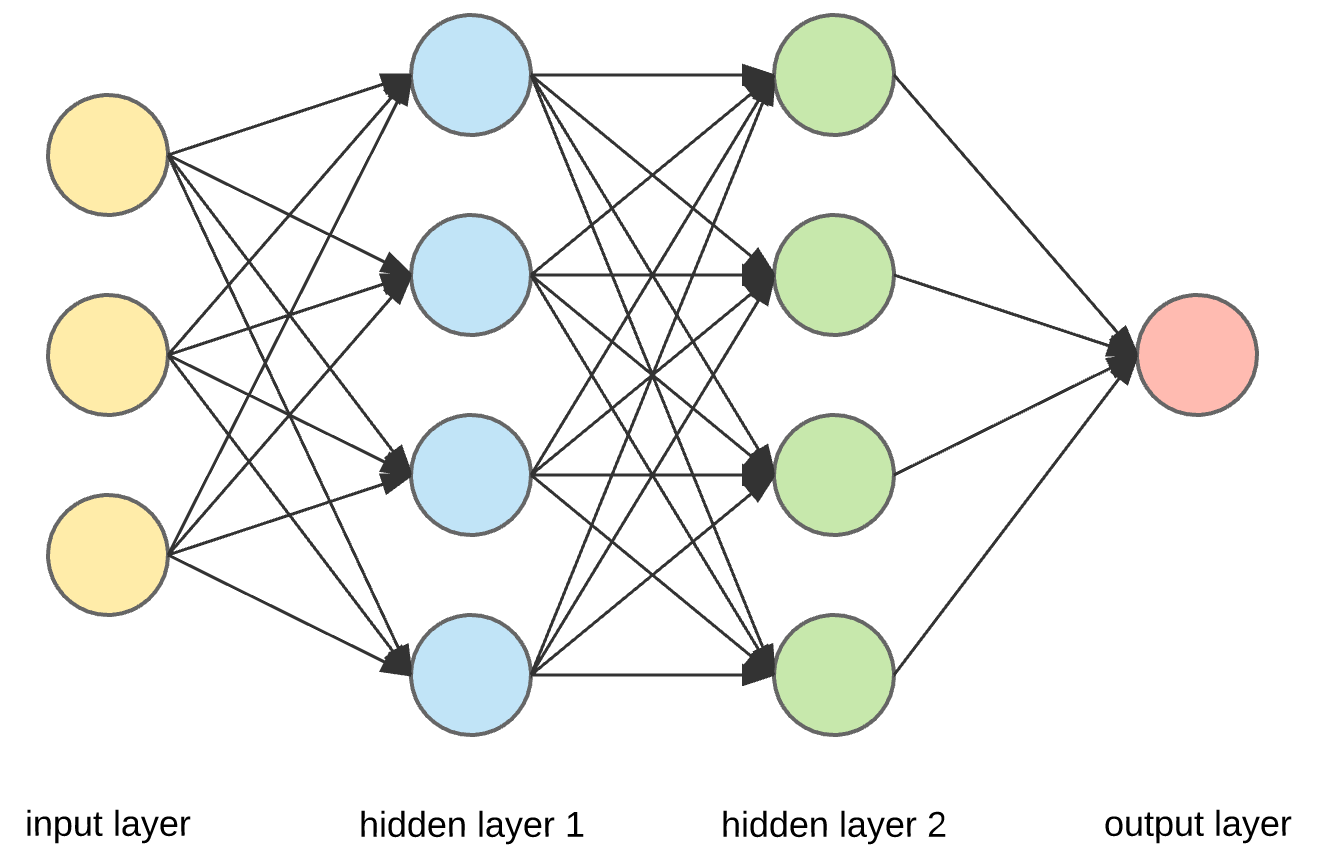
\includegraphics[width=\textwidth]{images/simpleNN.png}
				\caption{Schematic structure of the most basic fully connected deep neural network. Indicated are the input (yellow), output (red) and hidden layers (blue and green). Each neuron outputs to all neurons in the following layer, but there are no interconnection between neurons of the same layer. Note that while the network has the minimum depth (2 hidden layers) to qualify for a deep neural network, the width  could be smaller.}
				\label{Img_NNFully}
			\end{figure}

			%\todo{Funktionsweise}
			The working principle is to form a weighted sum $\sum_{i=1}^{N} w_{i,j} * x_{i}$ over the values from neurons of the previous layer $x_{i}$ weighted by the connecting weight $w_{i,j}$. The weighted sum is then evaluated by the activation function $\sigma()$ such that the new value $x_j = \sigma(\sum_{i=1}^{N} w_{i,j} * x_{i})$. Here i refers to the index of the neuron in the previous layer and j to the index of the neuron in the current layer.\\
			Since forming a weighted sum is a linear operation the activation function must be non-linear to enable the network to learn non-linear behaviour.\footnote{ref needed} The most common activation functions are the rectifier also called rectified linear unit (short ReLU) and exponential linear unit (ELU). Both are inspired by the asymmetrical behaviour of biological neural connections\footnote{reference needed}.\\
			%\todo{Describe training cycle}
		
			%\todo{Mention Convolutional to contrast}
			In contrast to fully connected networks convolutional networks apply a so called filter to the input. These filters consider the inputs of nearby neurons as well. They are usually used in image recognition and require data that has information stored in patterns, most commonly special patterns as in images. Fig. \ref{Img_NNConv} depicts an exemplary convolutional network for image data and gives indication to it's working procedure.
		
			%\begin{figure}
			%	\missingfigure[figwidth=0.5*\textwidth]{Picture depicting exemplary Dense NN}
			%	\caption{Exemplary Conv NN}
			%	\label{Img_NNConv}
			%\end{figure}
		
		\subsection{Structures}
			
		 
		\subsection{Hyper parameters}
			\label{HyperPar}
			A hyper parameter refers to a parameter of the network that is not changed during training. Since these can have substantial influence on the performance of the network they will be explained in the following
			\subsubsection{Depth}
				The depth of the network correlates directly to the amount of chained non-linear functions. Therefore it strongly influences the ability of a NN to learn abstract patterns. The more complicated a pattern is the more depth is "required" to learn the pattern. For example a simple classification between left and right only requires a shallow network, whereas recognizing different brands of car requires a deeper network.
			\subsubsection{Width}
				The width of a layer refers to the amount of neurons in that layer. Often networks are build of layers with the same width in each hidden layer. If that is the case one sometimes speaks of the width of the network which is then equivalent to width of a/each hidden layer.
			\subsubsection{Activation or Activation Function}
				As previously discussed the activation function introduces non-linearty to the network. Some activation function will be better suited to model a certain problem than others. If information about the model or pattern to be predicted is known, an activation function close to this will have better performance. For example predicting outcome of a sine function will perform better with exponential activations or uneven polynomial activations than even polynomials.%\todo{citation needed}
			\subsubsection{Loss Function}
				Choosing a loss function determines what criteria the network optimizes for which directly corresponds to which patterns it learns. For prediction one typically chooses a root mean square function. For classification cross entropy loss functions are most common.
			\subsubsection{Batch size}
				The Dataset is divided into subsets called batches which are fed to the current network during training. After each batch the weights are adjusted. Splitting the dataset in this way is advantageous to the computational performance during training. Less memory is used during training and the number of epochs trained is reduced. The flip side of using a batch size smaller than the number of training data is that the gradient for optimization will be worse in comparison to the gradient calculated with the full data set. 
			\subsubsection{Epochs}
				An epoch describes a full training cycle of training, validating and adjusting weights for the entire training data set. If the batch size is smaller than the number of training points then multiple\footnote{Number of batches in one epoch = rounded up $\left(\frac{Amount of Training Data}{Batch Size}\right)$} adjustments are made.%\todo{recheck wording}
			\subsubsection{Metrics}
				Metrics are additional information gained from the network during training and evaluation. Metrics are not hyperparameters since they do not influence the resulting network but are an important source of information for further improving the network structure. For example a secondary loss function can be implemented as a metric to evaluate general optimization of the network in contrast to only the chosen loss quantity. 
			\subsubsection{Regularization}
				%\todo{cite https://www.analyticsvidhya.com/blog/2018/04/fundamentals-deep-learning-regularization-techniques/}
				Regularization describes methods used to reduce the generalization error but not the training error. Commonly used regularization methods include L1, L2, Dropout and Early Stopping regularization. L1 and L2 regularization is applied by adding a penalty term to the loss function. This requires initial knowledge of input influences. For example an image with bad resolution might have a larger penalty term applied than an image with high resolution. Dropout regularization and early stopping are used to prevent overfitting. Since the amount of parameters in the network is often on the same order of magnitude as the amount of training data, neural networks are prone to overfitting. Early stopping interrupts the training process as soon as the validation loss stops improving by a user set minimum delta. 
	\section{Gaussian Processes}
		\subsection{General Introduction}
		\subsection{GOGAP algorithm}
%	\section{NNGP ?}